% Drawing 142/06-2 -- folder 142, batch 06, archive page 105 (PDF page 106).
% Transcription: Deuxième figure. Même sphère ; un seul sommet sur chacun des cercles de $0$ et $\infty$, deux sur celui de $1$ ; flèches $\Lambda^\infty_+$, $\Lambda^0_+$, $\lambda^1_+$, $\lambda^1_-$, $a^\infty$ (de $0$ vers $1$), $a^0$ (de $1$ vers $\infty$). Légende : « 4 sommets, 1 relation, 6 flèches » ; dessous : « 3 cas ».
% Kind: quiver on the sphere minus three points (small circles and paths). Method 2 (schematic redraw from the facsimile). Status: ok.
% Notes: One vertex on the circles of 0 and infinity, two on that of 1; arrows Lambda^infty_+, Lambda^0_+ (whole circles), lambda^1_+-, a^infty (0 to 1), a^0 (1 to infinity); a pencil loop surrounds the figure. Legends "4 sommets, 1 relation, 6 fleches" and "3 cas".
% Coordinates: 1 unit = 1 mm = 1/100 of the crop width (bbox in page fractions: [0.524, 0.05, 0.884, 0.254]).
% Redrawn by Claude (claude-opus-5-5), issue #73, 2026-11-07; not checked by a human; not compiled (no TeX in the session).
% Rights: reproduces part of the work -- behind RENDER_TRANSCRIPTS, never published by itself.
\documentclass[tikz,border=3pt]{standalone}
\usepackage{amsmath,amssymb}
\usetikzlibrary{patterns,arrows.meta}
\tikzset{pencil/.style={black!45}, struck/.style={black!35}, mark/.style={circle,draw,inner sep=1.3pt}, pt/.style={circle,fill,inner sep=0.9pt}, opt/.style={circle,draw,fill=white,inner sep=1.1pt}}
\begin{document}
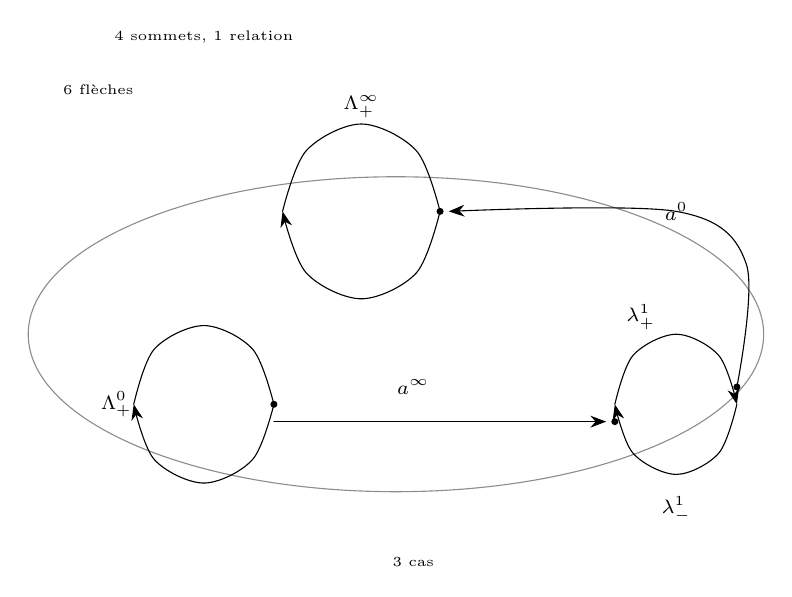
\begin{tikzpicture}[x=1mm,y=1mm,line cap=round,line join=round,font=\scriptsize]
\draw[pencil] (51.1,-48.9) ellipse[x radius=46.7, y radius=20];
\draw plot[smooth, tension=0.55] coordinates {(36.7,-33.3) (39.7,-25.6) (46.7,-22.2) (53.7,-25.6) (56.7,-33.3)};
\draw[-{Stealth[length=2mm]}] plot[smooth, tension=0.55] coordinates {(56.7,-33.3) (53.7,-41.1) (46.7,-44.4) (39.7,-41.1) (36.7,-33.3)};
\draw plot[smooth, tension=0.55] coordinates {(17.8,-57.8) (20.4,-50.8) (26.7,-47.8) (32.9,-50.8) (35.6,-57.8)};
\draw[-{Stealth[length=2mm]}] plot[smooth, tension=0.55] coordinates {(35.6,-57.8) (32.9,-64.8) (26.7,-67.8) (20.4,-64.8) (17.8,-57.8)};
\draw[-{Stealth[length=2mm]}] plot[smooth, tension=0.55] coordinates {(78.9,-57.8) (81.2,-51.6) (86.7,-48.9) (92.1,-51.6) (94.4,-57.8)};
\draw[-{Stealth[length=2mm]}] plot[smooth, tension=0.55] coordinates {(94.4,-57.8) (92.1,-64) (86.7,-66.7) (81.2,-64) (78.9,-57.8)};
\node[pt] at (56.7,-33.3) {};
\node[pt] at (35.6,-57.8) {};
\node[pt] at (78.9,-60) {};
\node[pt] at (94.4,-55.6) {};
\draw[-{Stealth[length=2mm]}] (35.6,-60) -- (77.8,-60);
\draw[-{Stealth[length=2mm]}] plot[smooth, tension=0.55] coordinates {(94.4,-55.6) (95.6,-40) (86.7,-33.3) (57.8,-33.3)};
\node[inner sep=1pt] at (46.7,-20) {\scriptsize $\Lambda^\infty_+$};
\node[inner sep=1pt] at (15.6,-57.8) {\scriptsize $\Lambda^0_+$};
\node[inner sep=1pt] at (82.2,-46.7) {\scriptsize $\lambda^1_+$};
\node[inner sep=1pt] at (86.7,-71.1) {\scriptsize $\lambda^1_-$};
\node[inner sep=1pt] at (53.3,-55.6) {\scriptsize $a^\infty$};
\node[inner sep=1pt] at (86.7,-33.3) {\scriptsize $a^0$};
\node[inner sep=1pt] at (26.7,-11.1) {\tiny 4 sommets, 1 relation};
\node[inner sep=1pt] at (13.3,-17.8) {\tiny 6 fl\`eches};
\node[inner sep=1pt] at (53.3,-77.8) {\tiny 3 cas};
\end{tikzpicture}
\end{document}
